\chapter{Dynamics of repetitive DNA}
\label{sec:DNA_sliding}
At first sight DNA with repetitive sequences seems to be a rather artificial concept and 
one would not expect such DNA to be relevant in biology.  
Consider a DNA sequence such as \basepair{5'-CACACACACACACACACACA-3'} and its complementary
counterpart \basepair{3'-GTGTGTGTGTGTGT\-GTGTGT-5'}. In a randomly assembled sequence of typical genome length 
the probability to find this particular sequence
%, or any sequence consisting of a two nucleotide motive repeated 10 times or more, 
is small (there are $4^{20}\approx10^{12}$ ways to assemble
a 20~bp sequence, a mammalian genome is about $10^9$~bps long and hence the chance of occurrence is on the order of $10^{-3}$).
\nomenclature{Genome}{The complete hereditary information of an organism encoded in DNA} 
Nevertheless, perfectly periodic sequences, \emph{i.e.~}repetitions of short motifs of one to six nucleotides, 
are extremely common in eukaryotic genomes \cite{Ellegren_NRG_04} 
and account for up to 3\% of the human genome \cite{HumanGenome_Nature_01}.
This drastic overrepresentation of repetitive sequences cannot be
linked to any particular function, since 
most of these repetitive sequences have been found in non-coding regions of the
genome. Instead, what makes repetitive DNA
special compared to ordinary DNA is its much richer dynamics. While two complementary
single stranded DNA molecules with a sequence that is not particularly ordered form base pairs
only when correctly aligned, repetitive sequences can bind out of register and form
asymmetric loops as illustrated in \FIG{repetitive_DNA}. In particular, two complementary
repetitive single strands can slip, meaning they can bind to each other when locally shifted. 
This phenomenon of DNA-slippage is the key to understand the peculiarities of repetitive DNA.
In the following, we will outline the role of repetitive DNA in biology and discuss how it is linked
to human hereditary diseases. 

%One part of this thesis is a theoretical study of the dynamics of repetitive DNA. 
Using a simple model
of repetitive DNA we explore the potential of single molecule experiments to study the dynamics of DNA 
slippage. Our theoretical analysis suggests, that DNA-slippage can be probed by applying a shear force to a 
repetitive dsDNA. We find that the two repetitive DNA strands start moving relative
to each other when a sufficiently high force is applied. The observed sliding speed 
can be related to the microscopic dynamics of DNA-slippage. 
%The theoretical description of DNA sliding makes use of many appealing concepts
%from equilibrium and non-equilibrium statistical physics.  
Hence, a thorough understanding of this sliding motion might give insight into 
 the molecular basis of DNA-slippage and shed light on the evolutionary dynamics
of repetitive sequences. The peculiar properties of repetitive DNA could also be exploited
in nanotechnology as visco-elastic elements and force generators. 
Our theoretical study is complemented by a collaboration with 
 the lab of Prof.~H.E.~Gaub, where Ferdinand K\"uhner and Julia Morfill succeeded in 
measuring DNA sliding using an atomic force microscope. These experiments are also discussed briefly.

Not only the  dynamical properties of repetitive DNA are different from ordinary DNA, but also 
its equilibrium thermodynamics is richer. If two repetitive and complementary DNA strands
of different length bind to each other, they undergo an additional temperature driven phase 
transition before they separate into two single strands at high temperatures. 
This additional transition will be discussed at the end of this chapter.

\begin{figure}
\centering
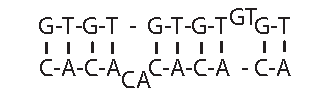
\includegraphics[width=\smallfigure]{\FIGPATH/Figures_sliding/repetitive_DNA}
\caption[Repetitive DNA has many binding configurations.]
{\label{fig:repetitive_DNA}
Two complementary DNA strands with repetitive sequence can bind in many different 
configuration, since strands are complementary even when locally shifted by in integral multiple of an 
repeat unit. In particular, repetitive DNA can form asymmetric loops and bulge loops, resulting in local strand slippage.
}
\end{figure}

\section{The biological role of repetitive sequences}
\nomenclature{SSR}{Simple sequence repeat. A multi-fold repetition of a short (one to six base pairs) motif\refpage}%
\nomenclature{Microsatellite}{Simple sequence repeat}%
\nomenclature{Short tandem repeat}{Simple sequence repeat}%
Repetitive sequences have first been observed in the early 80's \cite{Spritz_NAR_81} and since then 
have been found in every eukaryotic organism that was investigated. 
Repetitive sequences with short repeat motifs (one to six base pairs) are commonly 
called \emph{microsatellites}\footnote{DNA containing long repeated motifs forms 'satellite'
peaks in centrifugation experiments and such DNA was called satellite DNA. Later shorter and 
very short repeat motifs where observed and became known as mini- and microsatellites.}, 
\emph{simple sequence repeats} (SSR) or \emph{short tandem repeats}. To me, 
simple sequence repeat (SSR) appears to be the most natural name and I will try to stick to it.
Most of the simple sequence repeats are found in non-coding DNA and are believed to 
evolve more or less neutrally, that is the reproductive fitness of the organism is independent of length of the SSR. 
Only very little is known about possible functional roles of repetitive DNA, see below in \SEC{SSR_prokaryotes}. 
%While most SSRs appear to have no special function and are carried
%over time as ``selfish'' pieces of DNA, some people believe that SSRs have subtle roles in
%transcription regulation and might even be responsible for variability of socio-behaviorial traits
%\cite{Hammock_Science_05}. 
Within non-coding DNA, mono- and di-nucleotide repeats are
the most abundant, while within coding DNA, predominantly tri-nucleotide repeats are found.
Tri-nucleotide repeats constitute a special class of repeats, since the genetic code assigns amino acids to combinations of three bases, so called codons. 
\nomenclature{Genetic code}{Since there are more amino acids than bases, a multi-letter code is used to
store an amino acid sequence. Each amino acid is encoded by three consecutive bases, known as codons. 
The genetic code is redundant}%
A tri-nucleotide repeat in coding DNA therefore corresponds to 
a repeated amino acid in the protein. An extension or contraction of a tri-nucleotide repeat
results in the deletion or insertion of an amino acid but leaves other parts of the poly-peptide sequence 
unaltered. This is very different for most other repeat lengths, where expansions or deletions
result in frameshift mutations, \emph{i.e.~}the interpretation of the DNA sequence as three base
codons is changed for the entire part downstream of the repeat expansion. 
This most certainly results in a useless protein or premature termination of transcription. 
The special role of tri-nucleotide repeats and their 
relation to human hereditary diseases will be discussed in greater detail below.

\subsection{The number of repeats changes rapidly in evolution}
The key to understand the importance and ubiquity of SSRs
is the extraordinarily large rate at which the number of repeats changes from 
generation to generation. Although numbers have to be taken with care, rates
of contractions and expansions of SSRs in mammals can be as high as $10^{-2}$ per locus and
generation \cite{Dallas_MammGen_92}.
This is orders of magnitude higher than the typical rate for base substitutions which in mammals 
is about $10^{-9}$ per base and generation.	
This hyper-variability can be linked to a peculiarity of the mechanism by which DNA
is replicated prior to cell division. To replicate DNA, the double stranded molecule is
separated into two single strands by a helicase and the two single strands serve as
templates to which the complementary strands are added by the DNA polymerase. However,
the DNA polymerase operates only from the 5' to the 3' end. Therefore, only one strand,
the so called \emph{leading} strand, is copied continuously while the other strand, the \emph{lagging} strand, is
copied piecewise as illustrated in the upper panel of \FIG{replication_slippage}. 
The pieces of DNA that are added at a time
are known as \emph{Okazaki fragments}. The 5' end of an Okazaki fragment is fairly
unprotected and a couple of bases will frequently detach from the template strand by
thermal fluctuations. Whenever the 5' end of an Okazaki fragment happens to have a 
repetitive sequence, it is possible that it rebinds in a misaligned manner, forming a 
bulge loop containing one or more repeat units. 
\nomenclature{Okazaki fragment}{Piece of DNA polymerized continuously during piecewise replication of 
the lagging strand\refpage}%
If the DNA polymerase fills in the next Okazaki fragment while such a
bulge loop is present the number of repeat unit on the copied strand has changed with respect to the template strand. 
A bulge loop on the template strand  results in the deletion of one repeat, whereas a loop 
on the newly synthesized strand adds a repeat,
as illustrated in the lower panel of \FIG{replication_slippage}. 
%INDICATE TEMPLATE AND NASCENT STRAND IN FIGURE
\begin{figure}
\centering
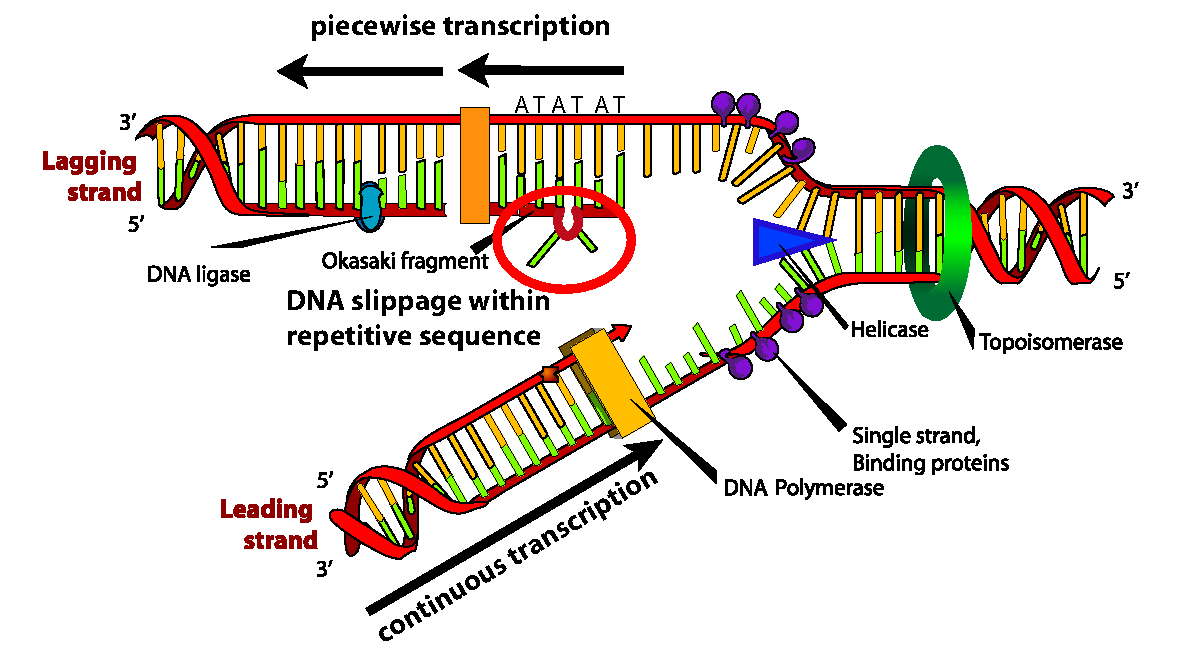
\includegraphics[width=\largefigure]{\FIGPATH/Figures_sliding/DNA_replication}
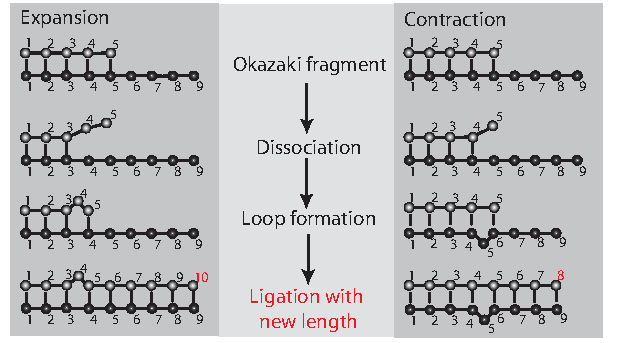
\includegraphics[width=\largefigure]{\FIGPATH/Figures_sliding/repeat_number_change}
\caption[Repeat number can increase or decrease during replication.]
{\label{fig:replication_slippage}
Upper panel: Replication of the lagging strand is done piecewise and the stretches replicated in one round
are called \emph{Okazaki fragments}. When an Okazaki fragment has a repetitive sequence,
the two strands can dissociate and subsequently rebind in a misaligned manner, as illustrated 
by the bulge loop inside the red circle. Image adapted from Wikipedia. Lower panel: Depending on whether the loop occurs on the template strand
or the new strand, the number of repeat units is increased or decreased in the copy.
}
\end{figure}

Energetically, SSR contraction is greatly favored over repeat expansion, since 
only one repeat unit has to open before a loop on the template strand can be formed, compared
to two repeat units that have to dissociate to from a loop on the nascent strand. 
Hence, one would expect SSRs to contract  and disappear quickly if the mutation mechanism was 
adequately described by the sketches in \FIG{replication_slippage}.
While this conclusion obviously contradicts
the abundance of SSRs in eukaryotic genomes, it explains the fact that SSRs are rare in prokaryotes and 
tend to contract during PCR, as discussed below in \SEC{PCR_slippage}.
The high ratio of expansion to contractions observed in eukaryotes is probably connected to the DNA mismatch repair machinery, which 
checks the double helical structure of the newly synthesized DNA. Only mutations
that escape this repair machinery or are falsely corrected persist to the next generation. Experiments in 
yeast have shown that a malfunctioning DNA mismatch repair system causes an increase 
of SSR mutations of 100-700 fold \cite{Strand_Nature_93}. These findings provide further indirect evidence that
misaligned rebinding during replication, \emph{i.e.}~replication slippage, is an important source of
SSR expansion and contraction. \emph{In vivo} rates of SSR evolution depend on a variety of different 
factors, most of which are still heavily debated in the literature. For a concise summary I recommend
\REF{Schloetterer_Chromosoma_00}.

\paragraph{SSR genesis and the length dependence of the mutation rate.}
The longer a SSR, the higher the probability that an open end during replication lies within
the SSR. One would therefore expect a linear increase of the expansion and contraction rate with
the number of repeats. Observations confirm a positive correlation between the 
repeat number and the mutation rate, the precise length dependence of the mutation rate, however,
is less clear and a large body of contradicting evidence exists (for a review, see \cite{Ellegren_NRG_04}).
Before a SSR can start growing by replication slippage, it has to contain at least two repeat
units.
% (If not convinced, try to redraw the replication slippage cartoons in \FIG{replication_slippage} for one, two and three repeat units.). 
It has been shown, that expansion of SSR does actually occur 
for SSRs as short as two units. It is generally believed that these initial seeds for SSR expansion are
assembled by chance.

\paragraph{Dependence of mutation rate on the repeat unit length.}
Another feature one would expect to have drastic effects on the SSR mutation rate, is the length of the
elementary repeat unit. The longer a repeat unit, the more bases have to dissociate before
DNA-slippage can occur. The activation free energy for DNA-slippage therefore increases
with repeat length and rates are expected to be small for SSRs with long repeat units. 
This reasoning is very well supported by \emph{in vitro} experiments (cf.~\SEC{in_vitro_slippage}),
but \emph{in vivo} evidence is less conclusive. Some experiments seem to confirm that
shorter repeat units mutate faster than long repeat units \cite{Lee_HumMolGen_99}. A bioinformatics
study also reports strongly decreasing mutation rates with repeat length \cite{Kruglyak_PNAS_98}. Repeated motifs
that are longer than five or six bases are not known to mutate significantly by replication slippage.

\paragraph{Length distributions of SSRs.}
A comparative study of the length distributions of SSRs of different repeat length in humans, mice, 
fruit-flies, and yeast revealed significant differences in abundance and distribution between different
organisms \cite{Kruglyak_PNAS_98}. In all cases, short SSRs are
most abundant. The longest SSRs are found in mice, but even for mice the frequency drops rapidly to zero 
beyond 40 repeats. The absence of very long SSRs is somewhat puzzling, since there appears 
to be a bias towards expansions of repeats\footnote{As noted above contractions are less costly energetically,
but more expansions seem to escape the mismatch repair machinery, resulting in an expansion bias.}. 
Furthermore, the mutation dynamics becomes faster as the length
increases. Very long SSRs are therefore expected. One possible resolution to this puzzle are point
mutations, which split a SSR into two smaller ones. The frequency of such a point mutation within one locus
increases with increasing length and thus provide a plausible explanation for stationary 
length distributions \cite{Kruglyak_PNAS_98}. However, one should keep in mind that many other influences, most importantly selection or unanticipated properties of the mismatch repair system, might be just as important
to understand SSR length distributions. 
%The issues, why short SSRs appear to expand but
%don't get arbitrarily long and how mutation properties differ between loci and across organisms
%is still far from resolved. 

The mechanism of SSR expansion discussed so far, \emph{replication slippage}, 
changes the length of an SSR usually by one repeat unit, sometimes by a few, but never by many.
However, the length of some special classes of SSRs tends to expand by a large number
of repeats in one generation. A common feature of such SSRs is their ability to form hairpins, 
\emph{i.e}~the ability of the single strand to fold back onto itself and form a stable structure.
Possible mechanism of SSR expansion due to hairpin formation are reviewed in 
\cite{Lenzmeier_CytoGenRes_03, Bzymek_PNAS_01}. Another source of length variations
of SSRs is unequal crossing-over during meiosis. When a diploid organism produces
haploid gametes, the genes on the chromosomes are reshuffled by building new chromosomes
out of pieces of the old ones. In repetitive parts of the genome, these recombination sites are 
ambiguous, which can give rise to two new chromosomes with SSRs of different length.


\subsection{SSRs are versatile genetic markers}
The human genome contains hundreds of thousands SSRs, each of which changes its length
with a probability of $10^{-6}-10^{-2}$ in each round of replication. The chance, that two humans
have the same set of SSRs is therefore negligibly small, even between closely related individuals. 
For this reason SSRs are ideally suited as genetic markers and have acquired great popularity
in phylogeny studies, paternity testing and forensic sciences. 
To measure the length of a set of SSRs, one exploits the fact that each SSR can be uniquely 
identified by its flanking sequences. A short fragment of DNA containing the SSR to be analyzed 
is cut from the sample using restriction enzymes that cut DNA specifically at the flanking sequences 
of the SSR. The short fragments are amplified by PCR and their length is measured using
gel electrophoresis. The resolving power of these
techniques is high enough to detect insertion and deletions of single repeat units \cite{Bennett_MolPath_00}. 
The great advantage of SSRs based genotyping techniques is the small length of the sequence 
fragments that need to be analyzed. Since short sequences can be efficiently amplified by PCR, 
minute DNA samples suffice for reliable data. 
Depending on the questions one wants to address, different genetic markers with different mutation
rates, chromosome type (autosomes, X-, or Y-chromosome) or flanking sequence are more 
suitable than others. 
\nomenclature{PCR}{Polymerase chain reaction. By PCR small amounts of DNA can be amplified rapidly and cheaply}
%Phylogenetic studies use the number of accumulated mutations as a molecular evolutionary clock
%to measure the time two species diverged from a common ancestor. For these applications a reliable 
%model and accurate parameters of SSR evolution have to be known to yield accurate predicitons.

\subsection{SSR expansion is related to hereditary diseases}
Most SSRs reside in non-coding regions of the genome and mutations of these SSRs
have little or no effect on the fitness of the individual. A special class of tri-nucleotide SSRs, however, occurs in 
coding regions or is part of introns, \emph{i.e.}~regions of a gene that are transcribed but spliced from the 
mRNA before translation, and mutations of these can lead to severely impaired phenotypes. 
Only tri-nucleotide repeats are found in coding regions due to strong selection against
frameshift mutations, which result by insertion or deletion of a number of bases that is incommensurate 
with three. Mutations of these tri-nucleotide SSRs are linked to a number of severe human hereditary
diseases, such as \emph{Huntington's}, \emph{fragile X} or \emph{Friedenreich's ataxia}.
These diseases fall into two different categories \cite{Reddy_COCEB_97}. 
The first class of tri-nucleotide related diseases is caused 
by expansions of \texttt{CAG} repeats that code for the amino acid glutamine. The most prominent
member of this class is Huntington's, which we will discuss in little more detail.
Huntington's is a neurodegenerative disease that develops gradually. At early stages, 
patients suffer from rapid uncontrollable movements. As the disease proceeds, 
patients loose virtually all motor control, including the ability to speak, eat, or facial expression. 
The gene containing the \texttt{CAG} repeat codes for the protein \emph{huntingtin}, whose
function is largely unknown. The number of repeats in healthy individuals ranges between 
6 and 34, people with 35 to 39 repeats have an increasing risk of developing the disease during
their lifetime and people with 40 or more repeats almost certainly suffer from Huntington's by the 
age of 40. Due to late onset of Huntington's disease, patients usually have children before
the disease is detected. The disease tends to becomes worse from generation to generation as the 
\texttt{CAG} repeat tends to grow longer and longer. The rate of elongation is correlated with 
the number of divisions in the paternal germ line \cite{Kandel_00}.
The molecular basis of the pathology of mutated huntingtin is still not completely 
resolved. The most popular hypothesis is, that proteins with a long poly-glutamine stretch tend
to aggregate and that those aggregates are toxic. Such aggregates have been found in the brains
of deceased patients. It is unclear, however, whether these aggregates are key to the pathology
or an unimportant byproduct \cite{Bates_Lancet_03}. In any case, it is extremely astonishing that 
the protein works fine with any number of glutamines between 6 and 34 and is almost certainly lethal 
with just 6 copies more.

The second class of pathological tri-nucleotide repeats are located in introns. In some
way or the other, the expansion of the SSR prevents transcription of the gene or the processing of the 
mRNA for translation into protein. 
Pathological expansions often reach repeat numbers as high as 2000, which is to be compared to the 
normal range of 5 to 50 \cite{Reddy_COCEB_97}. 
The most prominent member of this class is the fragile X syndrome causing mental retardation. 
Fragile X results from an expansion of a \basepair{CGG} unit beyond 200 repeats. 
The pathology of fragile X is believed to be related to methylation of \basepair{CG} di-nucleotides,
which might silence the transcription of the gene.



\subsection{SSRs in prokaryotes\label{sec:SSR_prokaryotes}}
In sharp contrast to eukaryotes, repetitive DNA is extremely rare in prokaryotes and
seems to occur only at loci, where there is a strong selective advantage to keep it. 
The prime purpose of SSRs in prokaryotes are \emph{contingency genes}, \emph{i.e.}~bacteria 
exploit the high mutation rate of SSRs to maintain genetic and phenotypic diversity within a 
population. Such diversity is essential to any organism subject to environmental 
changes, which may lead to extinction if not a small fraction 
of the population happens to be prepared for the new conditions \cite{Kussell_Science_05}.   
SSRs are exceptionally well suited for contingency genes, since SSR mutations are frequent and
lead to repeat number changes only. A change in repeat number differs from ordinary
base substitution mutations, since they are easily reversed. Assuming unbiased expansion
or contraction, there is a 50\% chance that a mutation is undone by the subsequent mutation, 
or put into more academic terms, random walks in one dimension are recurrent and almost surely
to return to the origin in finite time. This is very different for ordinary mutations, which correspond to 
a random walk in a very high dimensional space (every base can be of four different types), where
the chance of returning to a prior state is negligibly small. 

If there is a way to couple SSR contraction and expansion to switching genes on and off or 
to change protein function, rapid SSR mutations would result in phenotypic variation within 
populations and at the same time ensure easy recovery of temporarily switched off traits. 
Not surprisingly biology has found several ways to do so.
Among the best studied examples are contingency loci of human pathogens such as 
\emph{Haemophillus influenzae}\footnote{Although its name suggests that H.~influenzae
is the cause of the flu and hence a virus, H.~influenzae is a gram-negative bacterium. 
It was mistakenly associated with the flu until 1933.}
or \emph{Neisseria meningitis} \cite{Bayliss_JClinInv_01}. 
To evade the immune system,  these bacteria frequently exchange proteins in their outer 
membrane. This variability is often achieved by placing SSRs either in the promoter region or the in
coding sequence itself. A change in length within a promoter region can preclude necessary
interactions of transcription factors or destroy the RNA polymerase 
binding site. SSRs within the coding regions often cause frameshift mutations, which results 
in transcription termination or an ``gibberish'' mRNA. %In any case,  no functional protein is produced.


%\subsection{SSRs facilate homologous recombination}
%\cite{Napierala_JBC_02}



\subsection{\emph{In vitro} evidence for local strand slippage}
By now, it is fairly well established that replication slippage plays a pivotal role in the mutational
dynamics of SSRs. However, the change in repeat length from one generation to the next results
always from an interplay of replication slippage and the DNA mismatch repair machinery. Only
those mutations that escape mismatch repair or are falsely corrected can be detected. One way to study replication
slippage alone is to knock out the DNA repair machinery \cite{Strand_Nature_93}. Another way 
is to study DNA replication \emph{in vitro} \cite{Schloetterer_NAR_92}. Three examples of such 
experiments are described below.  

\paragraph{{\label{sec:PCR_slippage}PCR slippage.}}
The invention of the \emph{polymerase chain reaction} (PCR) was one of the most important steps
towards modern biotechnology. PCR allows to faithfully amplify minute amounts of DNA fast and cheaply.
During one cycle of PCR, the DNA template strands are separated by thermal denaturation, subsequently
the temperature is lowered such that short primer strands hybridize at the 3' ends of both strands.
A heat resisting DNA polymerase then extends the short primers and copies the template. By
multiple repetitions of these steps, the initial template is amplified exponentially.  
By now, PCR is a highly automated and very reliable technique. 
Only when amplifying repetitive DNA
the amplification is error prone \cite{Hauge_HumMolGenet_93, Murray_NAR_93}. The
product DNA is a mixture of the faithfully copied template DNA and DNA sequences where the
repetitive part has shortened by some repeat units. 
Why does the PCR loose repeat units while amplification?
%REDUNDANT....
Whenever the template strand has a repetitive sequence and the polymerase happens to fall
off the strand while transcribing the DNA, one strand can slip with respect to the other and 
form a bulge loop. Similarly to replication slippage \emph{in vivo}, the number of repeats changes 
if the polymerase resumes the replication while such a bulge loop
is present (cf. \FIG{replication_slippage}). 
Only contractions are observed due to the fact that the formation of a bulge loop has a lower
activation energy on the template strand.
Given a binding free energy per repeat unit $\eps$, contraction is more likely than expansion
by a factor of $e^{-\frac{\eps}{\kT}}$. 

\paragraph{\label{sec:in_vitro_slippage}SSR synthesis via DNA-slippage.}
\citeauthor{Schloetterer_NAR_92} succeeded in synthesizing repetitive sequences by exploiting 
DNA-slippage \emph{in vitro}. They mixed short repetitive DNA with DNA 
polymerase and the required nucleotides in a suitable medium. After some incubation time, 
they measured the length distributions of the DNA strands and found that the DNA
strands tend to grow \cite{Schloetterer_NAR_92}.  The elongation rate primarily depends 
on the length and the binding strength of the elementary repeat unit. 
Di-nucleotide repeats grow at a rate of 4 to 6 base pairs per minute while  tri-nucleotide repeats 
grow at a rate ranging from  0.5 to 3 base pairs per minute.
The elongation rate  of tri-nucleotide repeats correlates strongly with the number of 
\basepair{AT} base pairs in the repeat unit.

The observations can be explained by the following mechanism: 
The ends of the repetitive dsDNA undergo DNA-slippage and 
form a bulge loop which diffuses inside the double strand. The single stranded overhang
produced by this slippage event is then filled in by the DNA polymerase. When the
bulge leaves the double strand again, it
produces another single stranded overhang, which is then filled in by the
DNA polymerase. Since the rate of bulge loop formation depends exponentially on the 
binding energy of one repeat unit, di-nucleotide repeats are expected to grow faster than 
tri-nucleotide repeats. High \basepair{AT} content should also enhance slippage, as observed.

\paragraph{\label{sec:Poerschke}Evidence for chain sliding.}
In the 1970s, \citeauthor{Poerschke_BioPhysChem_74a} measured the hybridization kinetics
of short repetitive RNA oligomers \cite{Poerschke_BioPhysChem_74a}. 
When complementary strands are mixed, the rate limiting
step for hybridization is the formation of a critical nucleus of a few base pairs. Once such a 
nucleus is formed, the remaining bases rapidly close in a zipper-like manner. When sequences
have no particular order, a stable nucleus and subsequent zipping is only possible if the 
two strands are correctly aligned. This is very different for repetitive sequences,
since the two strands can bind with arbitrary shift relative to each other, see \FIG{Poerschke}a. 
Once such a misaligned duplex is formed, it is stable since both strands are bound by many 
base pairs. Hence, one would expect to find a large number of 
misaligned double stranded intermediates with a different number of base pairs.
The relaxation dynamics of these intermediates to the fully aligned state 
would further be expected to occur at markedly different rates, since 
the time required to dissociate the strands by thermal activation depends exponentially on the
number of base pairs. However, no such slow multi-exponential relaxation is observed 
\cite{Poerschke_BioPhysChem_74a}. 
\citeauthor{Poerschke_BioPhysChem_74a} himself provided a very plausible explanation 
for his results. As already discussed several times, repetitive sequences can form mobile
bulge loops. The propagation of a bulge loop from one end to another shifts both 
strands by the length of the loop, very much 
like a rug can be moved by propagating slack from one side to another, see \FIG{Poerschke}b. 
The energy cost for the nucleation of such a bulge is small and in particular does not depend
on the length of the molecule. 
\begin{figure}
\centering
\includegraphics[width=\smallfigure]{\FIGPATH/Figures_Sliding/Poerschke}
\caption[Evidence for fast chain sliding reaction.]{\label{fig:Poerschke}
Left: During the hybridization reaction of repetitive RNA oligonucleotides, many misaligned 
intermediates will be formed. Right: To explain the fast relaxation to the 
completely aligned state, \citeauthor{Poerschke_BioPhysChem_74a} suggested 
that the two strands can slide by the propagation of bulge loops from one end to the other.  
}
\end{figure}


\section{Force induced DNA-slippage}
The observations and experiments reported above provide good evidence that DNA-slippage
is indeed happening and that it plays a crucial role during SSR evolution.  
However, the evidence for DNA-slippage is more or less indirect and based on bulk 
observations. One goal of this thesis was to suggest experiments that allow to observe 
DNA-slippage in single molecules using modern force spectroscopy techniques (cf.~\SEC{force_spectroscopy}). 

We suggest, that  DNA-slippage can be induced by applying a shear force to 
repetitive DNA.  In a nutshell, application of a sufficiently high shear force fosters the 
formation of bulge loops on both unstretched ends of the DNA duplex, which then travel 
across the duplex and exit on the other side, as illustrated in \FIG{Poerschke}b. The duplex lengthens stepwise, 
where each step corresponds to an individual bulge loop,
the length of which can be one or several repeat units. We devise a theoretical model, that allows us
to predict experimental signatures and relate measurements to microscopic parameters of DNA-slippage.
Using kinetic Monte Carlo simulations, methods from statistical mechanics,
drift-diffusion, and reaction-diffusion theory, we uncover four different force regimes with
distinct characteristic behavior.
The model we use is simple enough to be amenable to analytic treatment, which
allows us to calculate the threshold forces and the average sliding speed exactly. 
We further investigate how this sliding behavior is affected by rare mutations that destroy
the perfect repetitivity of the sequence. Such mutations do not necessarily impede sliding,
but, depending on the frequency of such alien bases, delay the mechanical
response and require larger forces. 


%THEORY OF SLIDING
\subsection{Sliding dynamics of perfectly repetitive sequences}
In a typical force spectroscopy experiment, a force extension curve is recorded
until rupture. In such experiments, either the distance of the cantilever from the surface,
\emph{i.e.}~the extension of the sample, or the applied force is controlled, while the other is recorded.
Though in principle the same information can be gained from either of the two approaches,
there are significant practical differences between the two. 
The former is easier to implement experimentally, since distance can be precisely controlled
using piezo-elements. However, applying a constant force and monitoring extension is easier to interpret and handle analytically or numerically. In the following, we will study the response of repetitive dsDNA
to a constant shear force, as illustrated in \FIG{sliding_transitionstate}a.

\subsubsection{DNA sliding exhibits four different force regimes}
No matter how small forces are applied to the molecule, it will rupture eventually since the 
state of large separation has the lowest free energy. However, to separate the two strands, an activation
barrier has to be overcome. The height of this barrier depends on the applied force, as well as
on the internal dynamics of the system. In the case of repetitive DNA, the main question is whether
the two strands stayed in register or have shifted relative to each other before rupture.
Two possible transition states, \emph{i.e.}~the state prior to rupture, with and without sliding
are sketched in \FIG{sliding_transitionstate} b\&c. The free energies difference of these states to the
ground states are given by 
\begin{equation}
\label{eq:sliding_transitionstate}
\Delta E_{non-sliding}=N\left(\eps - f(\lss-\lds)\right) \quad \mathrm{and}
 \quad \Delta E_{sliding}=N\left(\eps - f(2\lss-\lds)\right).
\end{equation}
The parameters $\lss$ and $\lds$ are effective lengths of ssDNA and dsDNA chosen such that
the stretching free energy per base or base pair is given by $f\cdot\lss$ and $f \cdot\lds$, respectively.
Obviously, the transition state after sliding is always lower in free energy than the 
transition state, when both strands stick. At low force, however, even $\Delta E_{sliding}$
is positive and the dissociation of the two strands is a thermally activated barrier crossing process, no matter
which dissociation path is taken.
The rupture times are exponentially distributed with a mean time $\mrt$ that 
increases exponentially  with $\Delta E$ and hence exponentially with the length of the molecule. 
%Simulations confirm this reasoning, cf.~Fig.~2 in the publication reprinted in 
%\SEC{Neher_PRL_04}.
\begin{figure} 
\centering
\includegraphics[width=\largefigure]{\FIGPATH/Figures_sliding/transition_states}
\caption[Shearing repetitive DNA.]{\label{fig:sliding_transitionstate}
Part a): A dsDNA molecule sheared by a force $f$. Part b): When the DNA duplex ruptures without sliding, the last base pair before rupture will be a native base pair. Part c): If the two sequences
slide along each other, the transition state has a larger extension $L$, see text for details. 
Shorter duplexes rupture in a cooperative manner \cite{Strunz_PNAS_99}.
}
\end{figure}
The situation changes, when the force is increased to
\begin{equation}
\label{eq:sliding_fc_estimate}
\fc=\frac{\eps}{2\lss-\lds},
\end{equation}
where the $\Delta E_{sliding}$ ceases to be positive while  $\Delta E_{non-sliding}$
is still positive. If the duplex ruptures via sliding the dissociation should no longer be 
a thermally activated barrier crossing process but some sort of creeping motion from the ground state
to the transitionstate.  While sliding still involves local energy barriers such as bulge loop formation, 
there is no longer an extensive barrier. Hence, the mean rupture time no longer increases exponentially
with the length but is determined by how rapidly the two strands can move relative to each other. 
Simulations suggest, that $\mrt$ scales as $N^3$ at the critical force\footnote{
This force is actually slightly different from the expression given in \EQ{sliding_fc_estimate}
due to entropic effects.} $\fc$.
At forces above $\fc$, we observe a quadratic increase of $\mrt$ with $N$, see \SEC{Neher_PRL_04}.
How can the cubic and quadratic scaling be rationalized?
As suggested by \citeauthor{Poerschke_BioPhysChem_74a} the two strands can be shifted relative 
to each other by propagation of bulge loops from one end to the 
other end. But a loop that is nucleated at one end most likely leaves the duplex again at the same end.
It travels all the way to the other end only with probability $M^{-1}$, where $M$ is the  
number of base pairs (see \FIG{particles}a for illustration).
Since the nucleation rate of loops at the end is independent of the total length, the mobility of 
the two strands relative to each other is inversely proportional to the overlap length $M$.
This mechanistic explanation of strand mobility is consistent with the intuitive expectation, that
the friction coefficient of a one dimensional object should linearly depend on its length.
At the critical force, the nucleation rates of loops at stretched or unstretched ends are equal and 
the duplex shortens and lengthens at equal rates, resulting in an undirected diffusive motion.
Since the diffusion constant itself is inversely proportional to $N$, the time needed to overcome 
the distance $N$ increases as $N^{3}$. 
At forces above or below the critical force, bulge loops are 
nucleated more frequently on unstretched or stretched strands, respectively, than they are on the
opposite strand. This induces a directed motion either extending or contracting the duplex. The effective
drift velocity is inversely proportional to the overlap length $M$. The time required to overcome a
distance $N$ with a velocity proportional to $M^{-1}$ scales as $N^2$. 

This quadratic scaling does not persist to arbitrarily high forces, but crosses over to a linear
scaling. The threshold force $\fd$ for this crossover is given by the force, at
which also the $\Delta E_{non-sliding}$ becomes negative.
\begin{equation}
\label{eq:sliding_fc_unravell}
\fd=\frac{\eps}{\lss-\lds}.
\end{equation}
In this case, it is no longer 
energetically expensive to open base pairs from both ends. Since
consecutive opening of base pairs until rupture is faster than sliding, this 
mode of unravelling wins over sliding dynamically and repetitive sequences behave
similarly to random sequences. 

%%FIGURE illustrating particle anti-particle model?
\begin{figure} 
\centering
\includegraphics[width=\largefigure]{\FIGPATH/Figures_Sliding/particles}
\caption[Microscopic dynamics of DNA sliding.]{\label{fig:particles}
Left: A particle placed at site 1 will be exit at site $N+1$ rather than at site $0$ with probability $N^{{-1}}$. This 
can be seen from the steady state distribution resulting when particles are injected at a constant rate. 
The particle fluxes to the left or right are proportional to the slopes of the distribution, the ratio of which
is $N^{-1}$. 
Right: A particle-antiparticle model for bulge loop dynamics, see main text.
}
\end{figure}
On a macroscopic level, the sliding dynamics of the two strands is well described by a drift-diffusion
equation, where the drift and the diffusion coefficient are inversely proportional to the instantaneous
length $x$ of the overlap of the two strands at any instant. 
\begin{equation}
\label{eq:sliding_drift_diff}
\frac{\partial}{\partial t} \PD(x,t)=\frac{\partial}{\partial x} \left(\frac{D_0(f)}{x}\frac{\partial}{\partial x}-\frac{v_0(f)}{x}\right)\PD(x).
\end{equation}
By fitting the solution of this drift-diffusion
equation to the simulated rupture time distributions, we obtain the drift and diffusion 
coefficients $v_0(f)$ and $D_0(f)$ that
are independent of $x$ and depend on the force only. The dependence of the 
drift coefficient on the force can be understood by microscopic modeling of the bulge loop dynamics.
In essence, bulge loops on opposite strands behave as particles and anti-particles, cf.~\FIG{particles}b: They annihilate 
on encounter forming one double stranded repeat unit. Bulge loops can also be produced in 
pairs, when a spontaneously nucleated bubble separates into two bulges. The nucleation of bulge loops at the
ends is mimicked by a coupling to particle reservoirs, the density of which depends on the 
force applied to that particular end. The difference of particles and antiparticles fluxes is conserved and 
directly related to the sliding velocity of the two DNA strands: The sliding velocity is given by 
the difference of the reservoir densities on stretched and unstretched ends, 
divided by the length of the double stranded region. 
The reservoir densities are determined by the pseudo-equilibrium loop densities 
on stretched and unstretched ends, which be calculated from the partition sum of our 
model. These results and the corresponding plots are included in our publication entitled 
``Dynamics of Force-Induced DNA-slippage'' in \emph{Physical Review Letters} \cite{Neher_PRL_04}, which is reprinted in \SEC{Neher_PRL_04}. The details of the calculation of the partition sum, 
defect densities, and critical forces are presented in the \APP{DNA_partitionsums}.


%%EXPERIMENTS BY FERDI AND JULIA
\section{\label{sec:DNA_slippage_experiments}Single molecule experiments on DNA-slippage}
Our theoretical study was intended to trigger experiments that study DNA-slippage in single
molecules. We are very happy, that Ferdinand K\"uhner and Julia Morfill from the group of Hermann
Gaub were willing to perform such experiments and collaborate with us. 
The experiments show very clearly, that two strands with repetitive DNA can slide along each 
other once the applied shear force exceeds a certain threshold value. Sliding proceeds in  
stepwise manner and the observed steps are compatible with a shift by one repeat unit. 
The observations can be convincingly explained by the force induced formation of a bulge loop
which is propagated to the opposite end and thereby lengthens the duplex. 
The experiments were performed with two different sequences, a 10 fold repeat of 
\basepair{GTT} and a 15 fold repeat of  \basepair{GT}. 

In the vicinity of the threshold force $\fc$ for sliding, the sliding velocity is linearly related to $f-\fc$, 
and a sliding mobility $\mu$ can be defined via
\begin{equation}
\label{eq:sliding_mob}
v(f)=\mu \cdot(f-\fc)
\end{equation}
In the experiments the situation is reversed, as the velocity is imposed by the speed at which the 
cantilever is retracted and the force adjusts itself. Higher forces at a given speed correspond to 
higher ``friction'', \emph{i.e.}~lower mobility. The forces measured at different speed confirm an 
approximately linear relationship. As expected, the tri-nucleotide repeat
slipped slower than the di-nucleotide repeat.

The threshold forces observed in the experiments were considerably higher than expected
from theory. We expect this discrepancy to be the result of deformations of the duplex, which is
not accounted for by the theory. When a force is applied to one strand of dsDNA it will
take a few bases, probably of the order of one helical turn of the DNA, to distribute the force
evenly to both backbones. In this boundary region the double stranded structure is distorted. The
DNA sequences used are only 30~bps long and the two boundary regions take up the whole molecule. 
It is therefore not surprising, that the observed forces deviate from the theoretical estimates which
assume an undistorted structure. The short sequences also limited the number of possible
sliding steps to four or five\footnote{The terminal bases on both ends are opening and closing
very frequently and a duplex with fewer than 10~bp overlap rapidly dissociates under force before sliding
can be observed \cite{Strunz_PNAS_99}.}. Therefore, the predicted scaling behavior for the mean
rupture time could not be tested. Given the biological importance of repetitive sequences and 
putative applications as active nano-scale building blocks, mechanical properties and the 
kinetics of repetitive sequences continue to be an interesting and challenging field for 
single molecule studies. 
The publication containing these results is reprinted in \SEC{Kuehner_BiophysJ_07}
and the interested reader is referred to this publication for details \cite{Kuehner_BiophysJ_07}. 


%SLIDING WITH DISORDER
\section{\label{sec:sliding_disorder}DNA sliding in presence of sequence disorder}
After having discussed the sliding dynamics of perfectly repetitive DNA, the question whether
sliding is robust to mutations that destroy the repetitive pattern, arises naturally. We show that
DNA sliding persists even in presence of such disorder. However, the onset of sliding is delayed by a 
waiting time, during which all mutated base pairs are opened. 
 
To begin with, we simulated the response to a shear force of a molecule with repetitive 
sequence where once in a while a repeat unit has been exchanged by bases, that bind only to 
their native binding partner and not to any other bases in the sequence. We find, that 
the extension of the molecule remains constant for some time until suddenly a fairly normal 
sliding behavior sets in. The existence of some delay is obvious, since all mutated bases have to be opened before the molecule 
yields. But it is less clear how the state with all mutations open is established and how the delay
times are distributed. 
By monitoring the state of individual mutations during the waiting stage, we reveal that 
mutations open consecutively from both ends and that sliding starts, as soon as the last 
mutation has opened. The mechanism by which a mutation opens 
is illustrated in  \FIG{measuringrates}.


Since the mutations open from both ends of the molecule, the state of all mutations
can be described by the outermost mutations on both sides. If the total number of mutations
in the molecule is $M$, the outermost mutations perform a random walk on $[1,2,\ldots,M]$.
Sliding starts, when both of these random walkers meet, that is no more mutations are bound.
The rate, at which these random walkers hop, \emph{i.e.}~the outermost mutations open and close,
depends on the force and the spacing between mutations. At low force, the random walkers
are biased away from each other and mutations are preferentially closed. In this case, the 
waiting time before sliding increases exponentially with the size of the system. At high forces,
the mutations are preferentially open and the waiting time increases as a power law \cite{Schwarz_75}. 
We can therefore identify different dynamical regimes in the plane of 
mutation density and applied force, where rupture is fast or exponentially slow. 
%Mutations are driven open by the entropy gained when larger parts of the molecule are populated by 
%high loop densities. Conversely, mutations are kept closed due to the loss of base pairs and the
%formation of two permanent loops associated with the opening of a mutation. The mechanism, by 
%which mutations open and close is illustrated in \FIG{measuringrates}. The rates, at which the
%random walkers hop, \emph{i.e.}~at which the outermost mutations open and close, are therefore
%determined by the force applied and the spacing between mutations. Sliding starts, once the 
%outmost bound mutations coincide and the waiting time can therefore be modeled by the 
%first encounter of two random walkers in one dimension, where each site corresponds to one mutation. 
%When the two random walkers are biased away from each other, their typical time of first 
%encounter increases exponentially with the number sites, while they meet fast (polynomial) 
%if they are unbiased or biased towards each other \cite{Schwarz_75}. Indeed, the distributions
%of waiting times for evenly spaced mutations is well described by the random walker model. 
%Depending on the force and the mutation density, the waiting times either increase exponentially
%or polynomial with the length of the sequence, which allows us to extend the force regimes
%observed without mutations to weak sequence disorder. 

DNA sliding in presence of sequence disorder is treated in detail in our publication entitled ``DNA as a 
Programmable Viscoelastic Nanoelement'' in the \emph{Biophysical Journal} \cite{Neher_BioPhysJ_05}. 
Details of the two random walker model are presented in the supplementary material to this article. 
The publication and the supplementary are reprinted in \SEC{Neher_BiophysJ_05}.

%NANOSCALE BUILDING BLOCK
\section{\label{sec:nanomechanical_app}Repetitive DNA as a visco-elastic nanoelement}
In recent years DNA has become a popular material to build elaborate structures on a molecular scale
\cite{Seeman_Nature_03, Shih_Nature_04, Rothemund_Nature_06}. These applications exploit the
specificity of complementary base pairing to guide an ensemble of DNA strands with carefully designed
sequence into the desired conformation. DNA has also been used
to construct devices that undergo conformational transitions in response to a change in the
chemical composition of the environment. A very versatile approach is to construct strands that
bind competitively to a scaffold strand with different binding affinities. If the device is in a particular
conformation including a weakly binding strand, the addition of a more strongly binding strand 
will replace the weakly binding strand from the structure and, if designed properly, will result in the 
desired conformational change  \cite{Simmel_AppPhysLett_02}. Such competitive binding has also 
been used to reversibly cross-link acrylamid gels \cite{Lin_04}. Other structures are sensitive 
to variation of pH and such reversible pH-driven transitions have recently been coupled to an oscillatory
chemical reaction \cite{Liu_AngwChemie_03,Liedl_NanoLett_05}.

Here, we want to discuss briefly the potential of repetitive DNA in nano-mechanical applications.
Most applications mentioned above are rigid and conformational transitions occur only between 
well defined states or require the replacement of one strand by another. Repetitive DNA
might be useful when building more flexible devices that respond dynamically to mechanical forces. 
We have seen above that repetitive DNA lengthens by one repeat unit at a time, if subject to a 
sufficiently high shear force. Conversely, it contracts against a sub-threshold force until maximal
overlap of the two strands is reached. In this way, mechanical energy is reversibly transformed into
base pairing energy. Effectively, repetitive DNA acts as a contractile visco-elastic
element with a viscosity that can be programmed by choice of the length of the individual
repeat unit and the overall length of the molecule. The contractile force is determined by the
sequence composition. Such a visco-elastic element might find applications as a molecular tie-rope
that keeps a connection between two parts straight and at the same time adjusts its length. 
Another conceivable application is a molecular force sensor that responds to forces exceeding 
the threshold force. The read out signal could either be rupture or simply a relative
shift of the two strands measured by FRET. 
The sliding response can be delayed by mutations in the repetitive sequence that transiently
lock the two strands in a particular relative position. Cross-linking
 gels with repetitive DNA might also result in material with novel mechanical properties. 
A detailed characterization of the visco-elastic properties of repetitive DNA can be found
in the article reprinted in \SEC{Neher_BiophysJ_05} \cite{Neher_BioPhysJ_05}.

%INTERMEDIATE PHASE
\section{\label{sec:intermediate_phase}Intermediate phase in DNA-melting}
So far, we have been predominantly interested in dynamic features of repetitive
DNA, which proved to be much richer than DNA with sequences without a particular
order. Here, we show that not only the dynamics but also equilibrium properties of repetitive DNA 
are different from random DNA. 

The most prominent difference is, at least within Poland-Scheraga models,
 that the order of the melting transition is different for repetitive sequences than for ordinary sequences.
We have seen in \SEC{DNA_melting} that the order of the melting transition of DNA
depends on the entropy of denatured loops, which in turn is governed by the loop closure exponent $c$.
For random sequences, a loop of a given size at a given position corresponds to one
base pairing configuration. When sequences are repetitive, however, loops can be asymmetric
and the bases of a loop of size $n$ can be distributed between the two strands in $n+1$ ways.
This effectively reduces $c$ by one \cite{Poland_70}. 
Hence, no transition is observed if $c$ is smaller than 2, denaturation is continuous 
if $2\!\leq\! c\!<\!3$ and a first order transition is observed only, if $c\!\geq \!3$.
A brief discussion of physical values of $c$ was given in \SEC{DNA_melting}.

This argument can be formalized by calculating the partition sum of all possible pairings between
the two strands\footnote{Only pairings corresponding to alternating stems and loops (no crossing base pairs) 
are allowed. This is usually a good assumption due to steric constraints.}, as we already did to study DNA sliding. 
%Most of the theoretical
%studies of DNA denaturation consider only native binding of the two strands, partly because it captures
%the important features of the melting transition for most sequences, but also because
%it is easier to handle mathematically (for notable exceptions see \cite{Hill_JChemPhys_59,
%Garel_Biopolymers_04, Litan_JChemPhys_65}). For repetitive sequences, this simplification
%cannot be made and one has to generalize the model to all possible pairings between
%the two strands\footnote{Pairings are restricted to non-crossing base pairs, which 
%usually is a good assumption due to steric constraints.}.
%One finds, that repetitive sequences melt as ordinary sequences do, but the the loop
%closure exponent $c$ has to be replaced by $c-1$ \cite{Poland_70}. 
%Qualitatively, this is readily understood, since the bases of a loop of size $n$ can be 
%distributed in $n+1$ ways between the two strands, which a increases the weight
%of loops of this size by $\sim n$. Hence, no transition is observed,
%if $c$ is smaller than 2, denaturation is continuous if $2\!\leq\! c\!<\!3$ and a first order transition 
%is observed only, if $c\!\geq \!3$. The actual value of $c$ lies somewhere between 1.5 and 2.2, depending
%on how excluded volume effects are accounted for. A brief discussion of physical 
%values of $c$ was given in \SEC{DNA_melting}.
When the two strands have repetitive sequences, there is no reason to consider only strands of equal
lengths. Our study revealed an additional phase transition, which occurs when the two strands
are of different length. At low temperatures, the two strands form a rigid double
helix and the excess bases of the longer strand reside in a single stranded overhang. 
As the temperature rises, more and more of these unbound bases are absorbed into 
bulge loops within the double helix and the overhang becomes shorter. At a certain temperature
 all the bases are absorbed and the length of the overhang is no longer extensive. This transition
is a continuous phase transition which formally and conceptually resembles Bose-Einstein
condensation. The overhang corresponds to those particles that condense into the ground 
state, while bulge loops within the double helix correspond to populated excited states.
The intermediate phase persists in presence of weak sequence disorder. 
Our work on phase transitions in repetitive dsDNA is published
 in \emph{Physical Review E} \cite{Neher_PRE_06}, which is reprinted in 
\SEC{Neher_PRE_06}. 

\section{Conclusion \& Outlook}
The dynamics of repetitive DNA is a fascinating research area with many open questions 
remaining to be addressed. Due to their structural simplicity, such sequences are amenable to
methods from statistical mechanics and their generic properties can be elucidated 
without reference to a particular realization. We studied equilibrium and dynamical 
features of repetitive DNA using both analytical and computational tools. Many quantities such as
threshold forces, defect densities and phase diagrams can be calculated exactly within our model. 
When repetitive DNA  is sheared with sufficiently high forces the two strands start moving relative to each other. 
This motion is mediated by propagation of bulge loops from one end to the other, very similar to 
defect diffusion in crystals. The dynamics of the two strands can be described
by a drift-diffusion equation with drift and diffusion coefficients that are inversely proportional to 
the length of the double stranded overlap of the two single strands. The drift and diffusion coefficients 
can be related to the microscopic bulge loop dynamics using a reaction-diffusion model. These two 
different levels of description provide a link between the microscopic dynamics of a bulge loop inside 
double stranded DNA to the DNA sliding dynamics, that can be measured in single molecule 
experiments. First experiments confirm that two repetitive DNA strands slide relative
to each other when sheared \cite{Kuehner_BiophysJ_07}, but more experiments with longer strands are necessary to test the prediction
of different scaling regimes and to infer quantities such as bulge loop mobilities. 

From an engineering perspective, repetitive DNA has intriguing mechanical properties which could
be exploited in nano-scale devices. In essence, repetitive DNA acts as a visco-elastic element with 
a force offset. The characteristics of such an element can be chosen through sequence composition 
and length. By introducing mutations in the perfectly repetitive sequence, the response of the element
can be delayed in a controlled way.

The principle incentive to study repetitive DNA is to understand the evolutionary dynamics of simple
sequence repeats. Our research is focussed on microscopic properties of DNA under well controlled
conditions. On the other hand, the length distribution of SSRs in various 
genomes and the mutation dynamics \emph{in vivo} are being actively investigated. The gap between these too approaches is huge,
but I think that bridging this gap is not completely infeasible. After measuring the microscopic
rates in single molecule experiments, one can faithfully parameterize models for \emph{in vitro}
slippage as described in \SEC{in_vitro_slippage} \cite{Schloetterer_NAR_92}. By successively adding
a mismatch repair system, single stranded binding proteins, etc., it might be possible to understand
how these components work together \emph{in vivo}. 
Another possible role of DNA-slippage could be in prokaryotic transcription termination. 
Intrinsic terminator sequences in prokaryotes include a ``slippery" and weakly binding
poly-\basepair{A} stretch, usually 7 to 9 bases in length. Upstream of this of this slippery 
sequence is a palindromic sequence which forms a hairpin in the RNA transcript \cite{Hippel_Science_98}.
A popular hypothesis is, that this hairpin exerts a force on the RNA still inside the polymerase and
thereby terminates transcription \cite{Dalal_MCell_06}. The precise mechanism how this is happening is
unclear, but it is conceivable that the force exerted by the hairpin induces DNA-slippage, which then enables the
RNA to slide along the DNA out of the polymerase. It should be possible to address this question by pulling
on the nascent RNA strand as presented in \REF{Dalal_MCell_06} while having the polymerase transcribe 
repetitive and non-repetitive sequences with different binding energies.

%%%%PRL%%%
\cleardoublepage
\section[R.A.~Neher and U.~Gerland, \emph{Phys.~Rev.~Lett.}, {\bf 93}, 198102]{Dynamics of Force Induced DNA-slippage. R.A.~Neher and U.~Gerland, \emph{Phys.~Rev.~Lett.}, {\bf 93}, 198102, 2004}
\label{sec:Neher_PRL_04}
\clearpage
\addtocounter{page}{3}

%%%%FERDI_BIOPHYSJ%%%%%
\section[F.~Kuehner \emph{et al.}, \emph{Biophys.~J.}, {\bf 92}, 2491, 2007]{Force Induced DNA-slippage. F.~Kuehner \emph{et al.}, \emph{Biophys.~J.}, {\bf 92}, 2491, 2007}
\label{sec:Kuehner_BiophysJ_07}
\cleardoublepage
\addtocounter{page}{6}

%%%%%DISORDER_BIOPHYSJ%%%%
\section[R.A.~Neher and U.~Gerland, \emph{Biophys.~J.}, , {\bf 89}, p.~3846]{DNA as a programable visco-elastic nano-element. R.A.~Neher and U.~Gerland, \emph{Biophys.~J.}, , {\bf 89}, p.~3846, 2005}
\label{sec:Neher_BiophysJ_05}
\clearpage
\addtocounter{page}{9}

%%SUPPLEMENTARY MATERIAL
\subsection{\label{sec:biophysj_supp}Supplementary Material to \emph{Biophys.~J.}, {\bf 89}, p.~3846.}
\subsubsection*{Waiting Time Distributions}
\paragraph*{Two Random Walker Model}
We consider two random walkers in one dimension confined by two reflecting boundaries $M\!+\!1$ sites apart. Since we want to model the process of mutation opening preceding the sliding stage, we seek the distribution of times until encounter of both walkers, given they started at opposite boundaries. Their motion is equivalent to the motion of one walker on a triangular piece of the two dimensional square lattice.  The 2D walker on site $(m,n)$ corresponds the state, where the left 1D walker is $m$ steps from the left boundary and the right 1D walker $n$ steps from the right boundary (see Fig.~3, main text).  The 2D walker is reflected at the lines $m=0$ and $n=0$. The line, where both coordinates add up to $M-1$ corresponds to the cases, when both walkers in 1D meet and is therefore an absorbing boundary for the 2D walker. \\
The case, where the rates, at which the walker moves away and towards a boundary ($k_{in}$ and $k_{out}$) are independent of the site, has been solved by \citet{Schwarz_75} using the methods of image charges. \\ 
The quantity we are interested in is the distribution of the time of the first encounter of the two random walkers in 1D, or equivalently the lifetime distribution $P(\tau)$ of the random walker on the triangle. A walker sitting on any site $(m,n)$ with $m=M-2-n$ can hop on two absorbing sites with rate $k_{in}$. The distribution of $\tau$ is therefore given by
\begin{equation}
\label{eq:lifetime}
 P(\tau)=2k_{in}\sum_{n=0}^{M-2} \PD(n,M\!-\!2\!-\!n;\tau),
\end{equation}
 where $\PD(n,m;\tau)$ is the probability of finding the walker on site $(n,m)$ at time $\tau$, given it started at site $(0,0)$. In the following we derive approximations of the solution by \citeauthor{Schwarz_75}.

\paragraph*{Unbiased Hopping}
When the walker has no bias, e.g. $k_{in}=k_{out}=k$,  $\PD(n,m;\tau)$ is given by a sum of $4M^2$ terms. The solution by \citeauthor{Schwarz_75} can be rearranged to 
\begin{equation}
\begin{split}
  \PD(n,m;\tilde\tau)=&\frac{1}{M^2}\sum_{r,s=1}^{2M}e^{-2\tilde\tau M^2\left(2-\cos \frac{\pi r}{M}
-\cos \frac{\pi s}{M}\right)}(1-(-1)^{r+s})\\
&\cos\frac{\pi (2n+1)r}{2M}\cos\frac{\pi r}{2M}\cos\frac{\pi (2m+1)s}{2M}
 \cos\frac{\pi s}{2M},
\end{split}
\end{equation}
where  the time variable has been rescaled as $\tau=\tilde\tau M^2/k$. 
Only terms, where the argument of the cosines in the exponent are close to $0$ or $2\pi$, contribute significantly when $\tilde\tau>1/M^2$. After shifting the summation interval to $r,s=-M\ldots M\!-\!1$, significant terms are those the $r,s$ close to $0$. 
%Keeping only slowly decaying terms and rearranging the exponent, yields
%\begin{equation}
%\begin{split}
 % \PD(n,m;\tilde\tau)\approx&\frac{1}{M^2}\sum_{r,s=-M/2}^{M/2}e^{-4\tilde\tau M^2\left(\sin^2 \frac{\pi r}{2M}
%+\sin^2 \frac{\pi s}{2M}\right)}(1-(-1)^{r+s})\\
%&\cos\frac{\pi (2n+1)r}{2M}\cos\frac{\pi r}{2M}\cos\frac{\pi (2m+1)s}{2M}
 %\cos\frac{\pi s}{2M}.
%\end{split}
%\end{equation}
We can expand cosines with arguments $\frac{\pi r}{M}$ or $\frac{\pi s}{M}$ and keep only the first non-vanishing contribution.
\begin{equation}
  \PD(n,m;\tilde\tau)\approx\frac{1}{M^2}\sum_{r,s=-\infty}^{\infty}e^{-\tilde\tau\pi^2\left(r^2+s^2)\right)}(1-(-1)^{r+s})
\cos\frac{\pi (2n+1)r}{2M}\cos\frac{\pi (2m+1)s}{2M}.
\end{equation}
The range of summation can be safely extended to $\pm \infty$, as terms with big $r,s$ are exponentially small.
Plugging this approximation into \EQ{lifetime} yields, after some algebra, using similar approximations as above, 
\begin{equation}
 P(\tilde\tau)\approx\frac{2}{M^2}\sum_{r,s=-\infty}^{\infty}e^{-\frac{\tilde\tau\pi^2}{M^2}\left(r^2+s^2)\right)}\frac{(1-(-1)^{r+s})(r^2+s^2)}{r^2-s^2}
\end{equation}
Since only those terms with odd $r+s$ contribute, we change the summation variables to $2v=r+s-1$ and $2w=r-s-1$.
\begin{equation}
 P(\tilde\tau)\approx\frac{4}{M^2}\sum_{v=-\infty}^{\infty}e^{-\frac{\tilde\tau\pi^2}{2}\left(2v-1\right)^2}\frac{(-1)^{v}}{2v-1}\sum_{w=-\infty}^{\infty}e^{-\frac{\tilde\tau\pi^2}{2}\left(2w-1\right)^2}(-1)^{w}(2w-1)
\end{equation}
From this expression, we find a parameter-free lifetime distribution
\begin{equation}
  \tilde{P}(\tilde\tau)=M^2P(\tilde\tau)=-\frac{16}{\pi^2}\frac{\partial }{\partial \tilde\tau}Q(\tilde\tau)^2,
\end{equation}
where $Q(\tilde\tau)$ is given by
\begin{equation}
  Q(\tilde\tau)=\sum_{n=1}^{\infty}\frac{(-1)^ne^{-\frac{\pi^2 (2n-1)^2 \tilde\tau}{2}}}{2n-1}
\end{equation}
The approximations involved are justified for large $M$. However, even for small systems the 
agreement is excellent, as illustrated in \FIG{lifetime}.
\begin{figure}
\centering
\includegraphics[width=\smallfigure]{\FIGPATH/Figures_Supplementary/finite_size_J(t)}
\caption[Supp.: The lifetime distribution of two random walkers.]
{\label{fig:lifetime}The lifetime distributions for $M=3,5,10$ and the approximation for large $M$. The time axis is rescaled by $M^2$.}
\end{figure}

\paragraph{Biased Hopping}
When the rates $k_{in}$ and $k_{out}$ are different, there is no compact analytical expression for $\PD(n,m;t)$. However, the longterm behaviour of a such a biased random walker is easily understood. If $k_{in}$ is bigger than $k_{out}$, the walker approaches the absorbing boundary steadily. In the opposite case, the walker will stay close to the origin and only rare excursions will lead to absorption. Quantitatively, the hopping of the random walker on the triangle is well approximated by suitably chosen one-dimensional representation. To that end, we consider the probability to find the walker on the line $\nu$ steps away from the origin.
\begin{equation}
P(\nu;\tau)=\sum_{m=0}^{\nu}\PD(m,\nu\!-\!m;\tau)
\end{equation}
This amounts to projecting the motion of the random walker onto the symmetry axis of the triangle. 
The time derivative of this quantity is very similar to a one dimensional hopping process.
\begin{equation}
\begin{split}
\partial_\tau P(\nu;\tau)=-&2(k_{in}+k^{-})P(\nu;\tau)+2k_{in}P(\nu\!-\!1;\tau)+2k_{out}P(\nu\!+\!1;\tau)\\
&+k_{out}\left[\PD(0,\nu;\tau)+\PD(\nu,0;\tau)-\PD(0,\nu\!+\!1;\tau)-\PD(\nu\!+\!1,0;\tau)\right]
\end{split}
\end{equation}
The contributions from the boundary terms in the second line depend on the ratio of $k_{in}$ and $k_{out}$. 
When $k_{in}\gg k_{out}$ the walker rapidly approaches the absorbing boundary. The probability $\PD(0,\nu;\tau)$  of finding the walker on the reflecting boundary is small, as it is unlikely to make equally many steps with high rate and a low rate. In this case the boundary terms can be neglected entirely, so that the process reduces entirely to a 1D first passage problem. Using standard methods described in \REF{Gardiner_04}, one finds, that the mean first passage time 
\begin{equation}
\mt=\frac{M-1}{2k_{in}-2k_{out}}-k_{out}\frac{1-\left(\frac{k_{out}}{k_{in}}\right)^{M-1}}{2(k_{in}-k_{out})^2},
\end{equation}
increases linearly with the number of mutations $M$.  \\
In the opposite limit, when $k_{in}\ll k_{out}$, $\mt$ increases as $\left(\frac{k_{out}}{k_{in}}\right)^{M-1}$ with $M$. In this case equilibration along the line $n\!=\!\nu\!-\!m$ is fast compared to the lifetime of the walker and  $\PD(m,\nu\!-\!m;\tau)$ is almost independent of  $m$. Setting all terms $\PD(m,\nu\!-\!m;\tau)$ equal results in a 1D hopping process with site dependent rates. The mean first passage time of this process can be calculated in much the same way, yielding $\mt\sim \left(\frac{k_{out}}{k_{in}}\right)^{M-1}$ with polynomial corrections.
In summary, we find that, depending on whether the walkers have an inward bias, an outward bias or no bias, the mean lifetime scales linearly, exponentially or quadratically with time.
Since the force, at which $k_{in}$ and $k_{out}$ are equal, separates regimes, where the waitingtime increases exponentially with $M$ from  linear scaling, we call it critical
force $\tfc$ in the presence of mutations. The force  $\tfc$ 
converges towards the critical force $\fc$ in the limit of no mutations.


\subsubsection*{Measuring Hopping Rates}
So far, we have been concerned with the waitingtime distribution given a certain set of rates, at which mutations open or close. These rates depend on the applied force and on the distance between consecutive mutations and have to be determined in simulations. 

As long as there are at least two mutations bound, the dynamics of the opening and closing of mutations at one end is independent of the other end. To measure the rates for a given pair of force and mutation density, we used a simplified system,
where a dsDNA with equidistant mutations is fixed on the right hand side
and a force is applied to the first base of the upper strand 
(see \FIG{measuringrates}). This simplified system is useful, as finite size effects are smaller when one walker crosses $M$ mutations as when two walkers cross $M/2$ mutations each. Furthermore, subtleties of the mutual annihilation process do not enter the measurement.
\begin{figure}
\centering
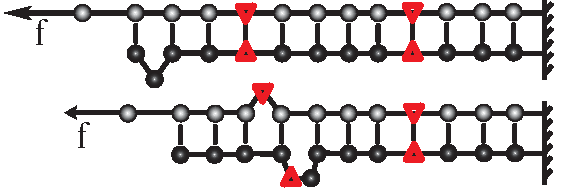
\includegraphics[width=\smallfigure]{\FIGPATH/Figures_Supplementary/Mutation_twostate}
\caption[Supp.: Measuring rates of mutation opening and closing.]
{\label{fig:measuringrates}Simplified system to measure the opening
and closing rates of mutations. The simulation starts from the ground state
with all bases bound. We determine the first-passage time distributions
of the opening of the rightmost mutation and fit these to a the first passage
time distribution of a random walker.}
\end{figure}
We measure the distribution of the time it takes to open the rightmost mutation for the first time and fit this distribution to the lifetime distribution of a random walker in one dimension between reflecting and absorbing boundary conditions. The rates $k_{in}$ and $k_{out}$ are fit parameters. This is done for a range of forces and mutation densities and the critical force $\tfc$ for a certain mutation density can be extract from the crossing of $k_{in}$ and $k_{out}$. To further pin down $\tfc$, we generated data for many force values slightly above and below $\tfc$ and fitted a linear relation for each rate to all data sets simultaneously. The crossing of the two resulting lines yield a robust estimate of $\tfc$. 
Using a system of $N=240$ basepairs, energy parameters $\eps=1.11\kT, \Eini=2.8\kT$ and different number of equidistant mutations, we determined $\tfc$ over broad range of mutation densities. The results are shown in Fig.~7(c) in the main text. \\
To check the reliability of the estimation of $\tfc$, we simulated waitingtime distributions by applying the force to both ends of the DNA and fitted the two random walker model to the waitingtime distribution. The force, where $k_{in}$ and $k_{out}$ coincide, reproduces the previously determined force $\tfc$. Furthermore, fitting the critical distribution (one fit parameter)  to the waitingtime distribution with yields best fits for $f\approx \tfc$. The absolute value of the rates shows slight dependencies on the length of the system (see below) and varies for fits to different setups. \\

\paragraph{Caveats of the Model}
Equilibration of the loopdensity is only possible by propagation of loops from the end beyond a newly broken mutation, or in other words by sliding the unstretched strand some distance $\Delta d$ inward. The sliding velocity, however,  is inversely proportional to the length of the strand. Therefore, equilibration will slow down breaking of mutations for supercritical forces deep inside the double strand and the linear dependence of the waitingtime on the number of mutations  will not persist for very large systems.

It is clear from the microscopic mechanism leading to breaking and opening of mutations (see main text and \FIG{loopdensities}) that the rates $k_{in}$ and 
$k_{out}$ depend on the force $f$. The rate $k_{out}$ also depends on the mutation density, since a great distance between mutations corresponds to a large entropy barrier for mutation closing, and hence a smaller closing rate $k_{out}$. The microscopic opening rate $k_{in}$ is expected to be more or less independent of the mutation density. When looking at the opening and closing dynamics of an individual mutation, this is what we observe.
However, the equilibration of loop densities after an opening or closing event takes some time. Therefore, successive microscopic opening and closing events are not entirely uncorrelated, which makes an unambiguous definition of the microscopic rates difficult. These correlations die out very quickly and it is still possible to describe the observed lifetime distribution with an uncorrelated random walker. The effective rates describing this motion both depend on mutation density and the applied force.

\begin{figure}[htb]
\centering
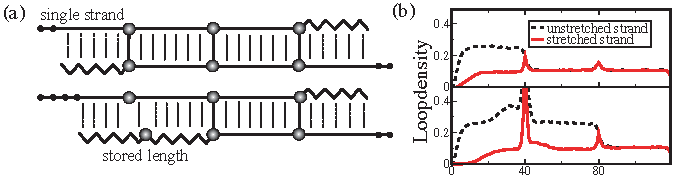
\includegraphics[width=\smallfigure]{\FIGPATH/Figures_Supplementary/loopdensities}
\caption[Supp.: Mutation opening is a trade-off between entropy and energy.]
{\label{fig:loopdensities}
Left: Illustration of how the density of loops on the strands depends on the state of the mutated bases in the sequence. In between bound mutations loops are rare, as the formation of a loop costs initiation energy and shortens the system. The same applies to the stretched strands outside bound mutations. The only part, where a significant number of loops can be found, is the unstretched strand outside the bound mutations. When a mutation is broken, loops  move across the mutation on the unstretched strand and locally both strands are shifted against each other. Thereby, the bases that previously formed the mutated basepair become permanently separated and the single strand part on the stretched strand grows.  
Right: To support the cartoon-like picture of part (a), we measured the time averaged loopdensity, conditioned on a certain mutation state.
Mutations are located at base 40 and 80, the parameters are $\eps=1.11\kT$, $\Eini=2.8\kT$ and $f=10.7 \pN$. We consider only opening of mutation from the left, i.e. the rightmost base is kept fixed, as in \FIG{measuringrates}. 
When all mutations are bound (upper panel), the loopdensity is high only on the unstretched
strand to the left of the mutation at position 40. When this mutation is broken (lower panel), loops can spread from the left end to the mutation at position 80, yielding a fairly constant density interrupted only by the permanent loop at the position of the mutated base. The hump to the left of the broken mutation on the unstretched strand and to the right of the broken mutation on the stretched strand indicate the position of the mutated base on the opposite strand. A loop already present on one strand renders unbound bases on the other strand more likely, as no additional loop initiation has to be paid. The vanishing loopdensity at the end of the stretched strand indicates unbound ssDNA. Observe, that this is the longer, the more mutations are broken. }
\end{figure}
\cleardoublepage
%%%%%INTERMEDIATE PHASE PRE%%%
\section[R.A.~Neher and U.~Gerland, \emph{Phys.~Rev.~E}, {\bf 73}, 030902(R)]{Intermediate phase in DNA-melting. R.A.~Neher and U.~Gerland, \emph{Phys.~Rev.~E}, {\bf 73}, 030902(R)}
\label{sec:Neher_PRE_06}
\clearpage
\addtocounter{page}{3}


